\documentclass[aspectratio=169,11pt]{beamer}

\usetheme{Boadilla}
\usecolortheme{default}
\setbeamertemplate{navigation symbols}{}
\setbeamertemplate{footline}[frame number]

\usepackage[T1]{fontenc}
\usepackage{graphicx}
\usepackage{amsmath,amssymb}
\usepackage{xcolor}

\definecolor{accentblue}{RGB}{30,70,140}
\setbeamercolor{title}{fg=accentblue}
\setbeamercolor{frametitle}{fg=accentblue}
\setbeamercolor{structure}{fg=accentblue}

\title{Fourier Synthesis and Gibbs Phenomenon}
\subtitle{CMPE362 Homework 2}
\author{Ali Ayhan G\"under \\ 2021400219}
\institute{Bo\u{g}azi\c{c}i University \\ Department of Computer Engineering}
\date{Spring 2026}

\begin{document}

\begin{frame}
  \titlepage
\end{frame}

\begin{frame}{Square Wave: Multiple Approximations ($N=5,20,100$)}
  \centering
  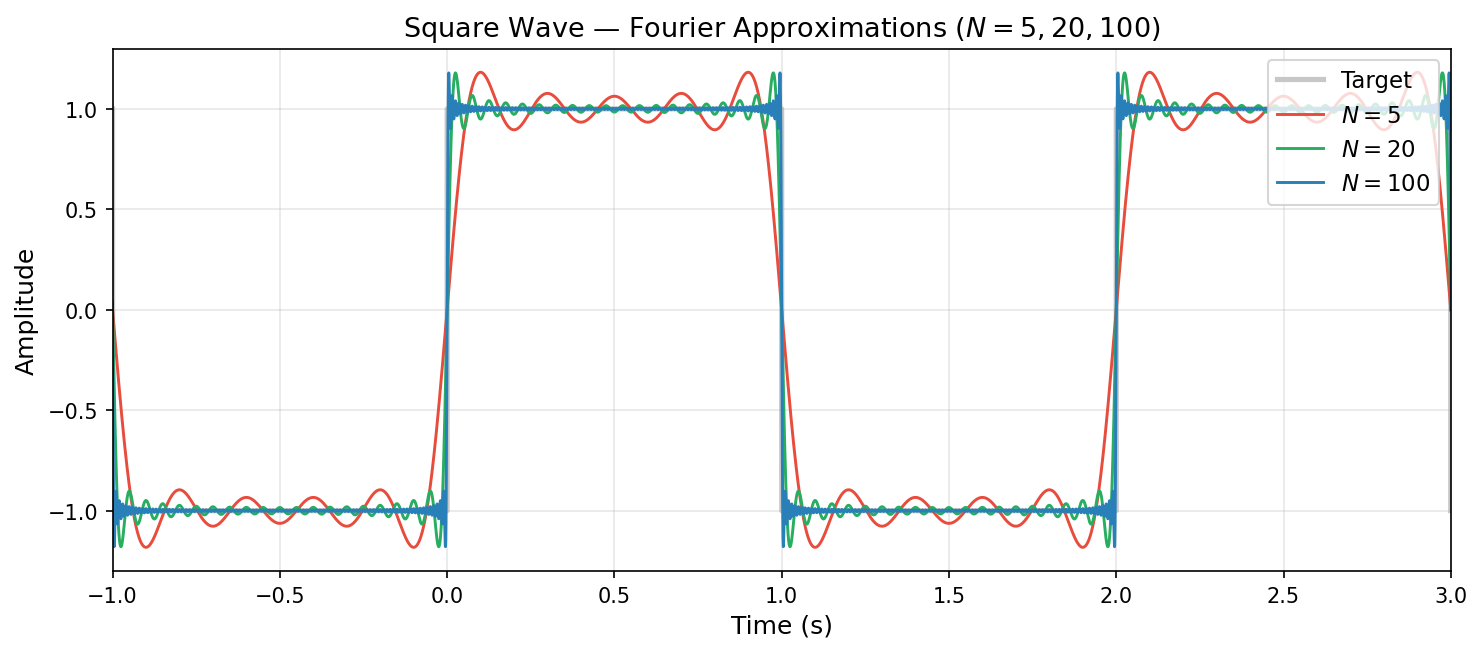
\includegraphics[width=\textwidth,height=0.85\textheight,keepaspectratio]{sq_full.png}
\end{frame}

\begin{frame}{Square Wave: Gibbs Phenomenon (Zoom Near Discontinuity)}
  \centering
  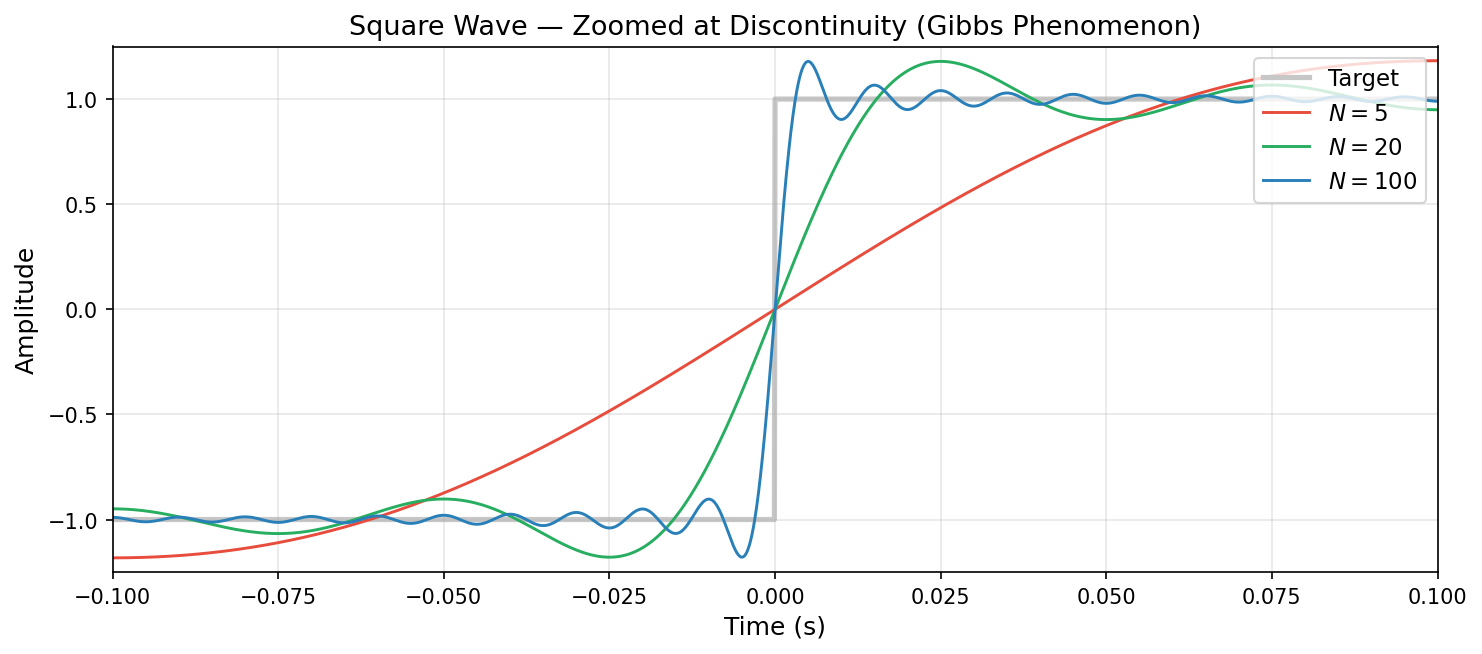
\includegraphics[width=\textwidth,height=0.85\textheight,keepaspectratio]{sq_zoom.png}
\end{frame}

\begin{frame}{Triangular Wave: Multiple Approximations ($N=5,20,100$)}
  \centering
  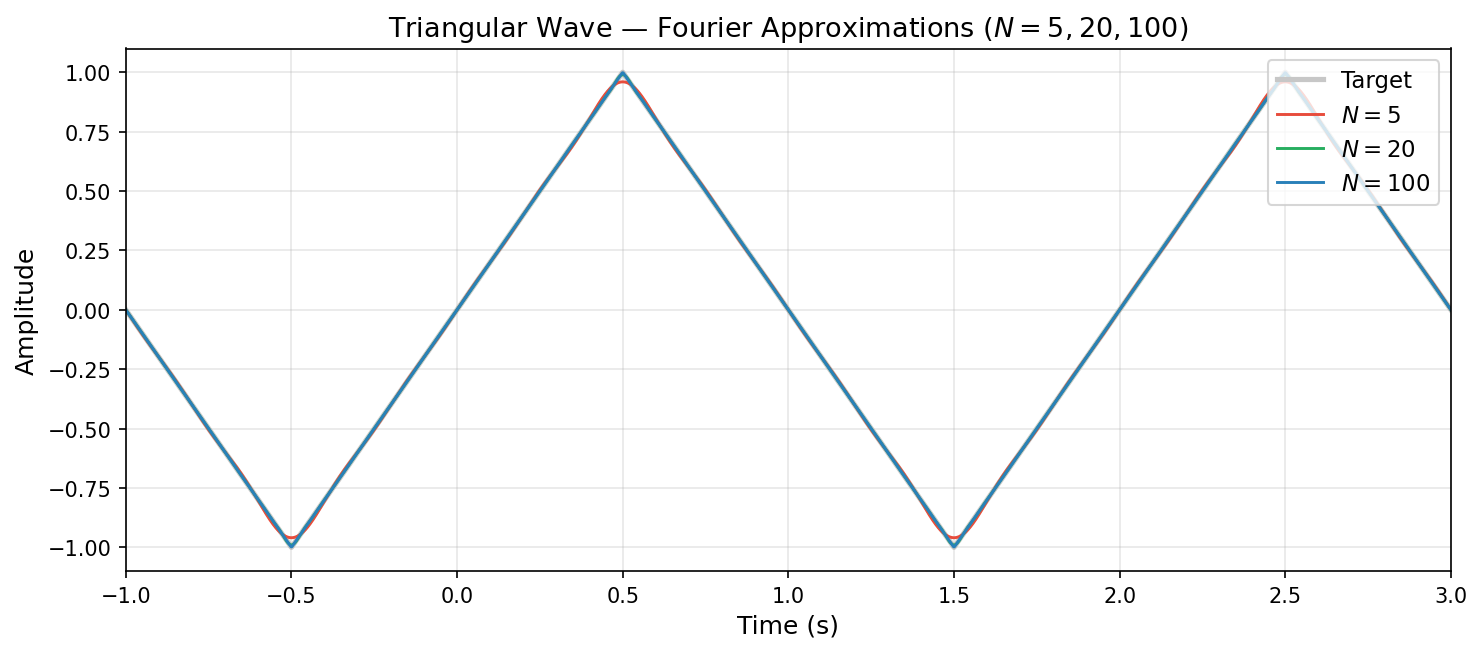
\includegraphics[width=\textwidth,height=0.85\textheight,keepaspectratio]{tri_full.png}
\end{frame}

\begin{frame}{Triangular Wave: Zoom Near Peak}
  \centering
  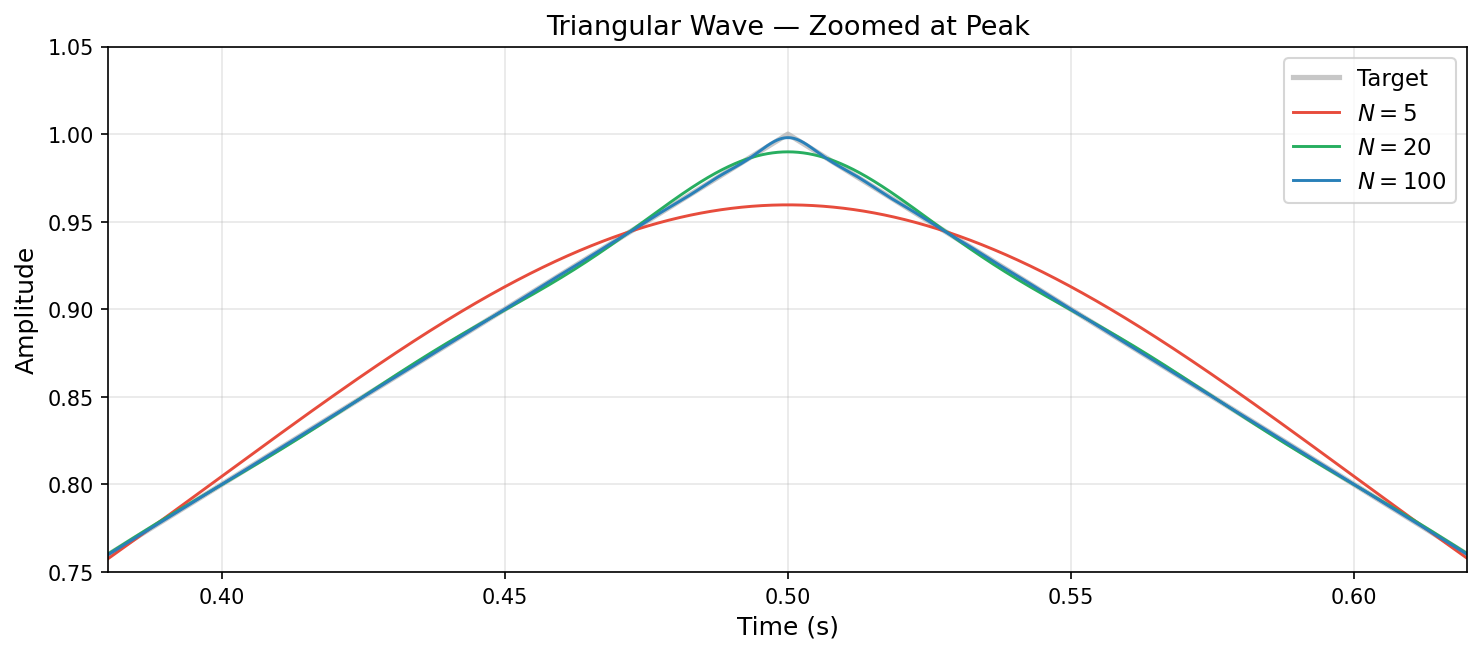
\includegraphics[width=\textwidth,height=0.85\textheight,keepaspectratio]{tri_zoom.png}
\end{frame}

\begin{frame}{Full-Wave Rectified Sine: Multiple Approximations ($N=5,20,100$)}
  \centering
  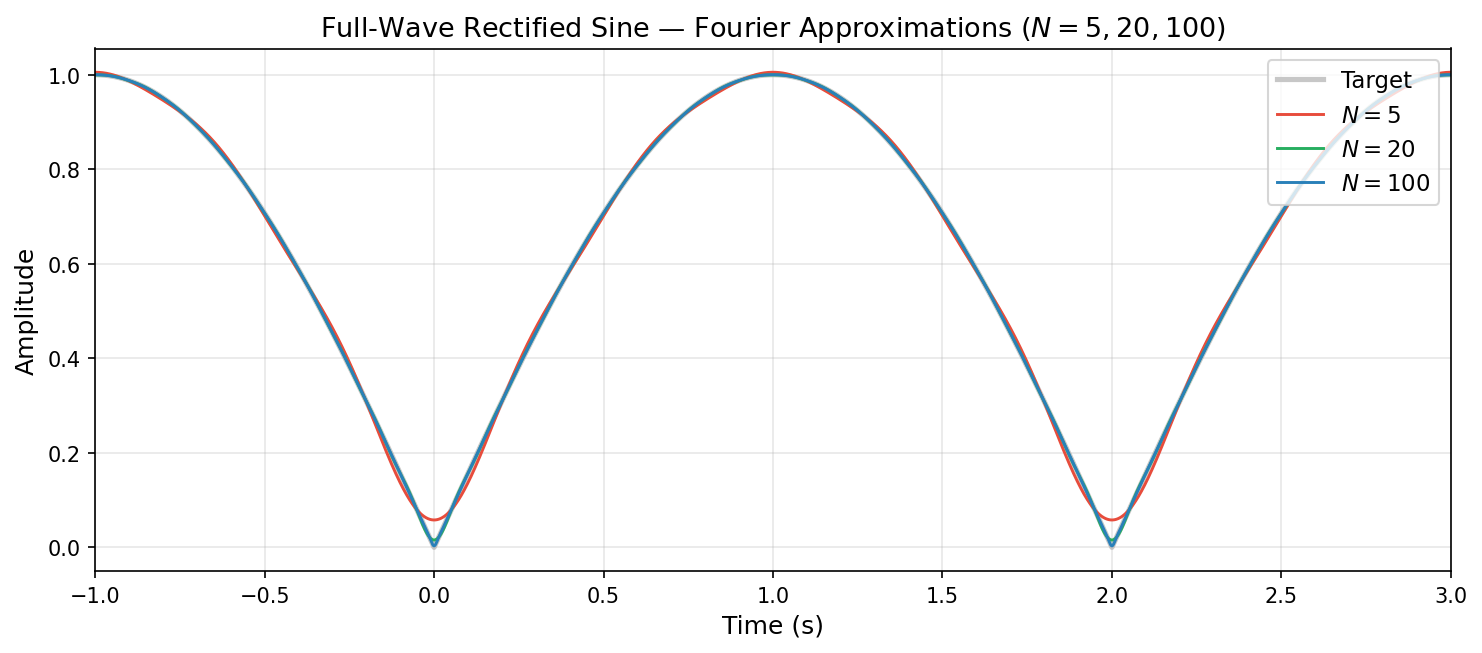
\includegraphics[width=\textwidth,height=0.85\textheight,keepaspectratio]{rect_full.png}
\end{frame}

\begin{frame}{Full-Wave Rectified Sine: Zoom Near Cusp}
  \centering
  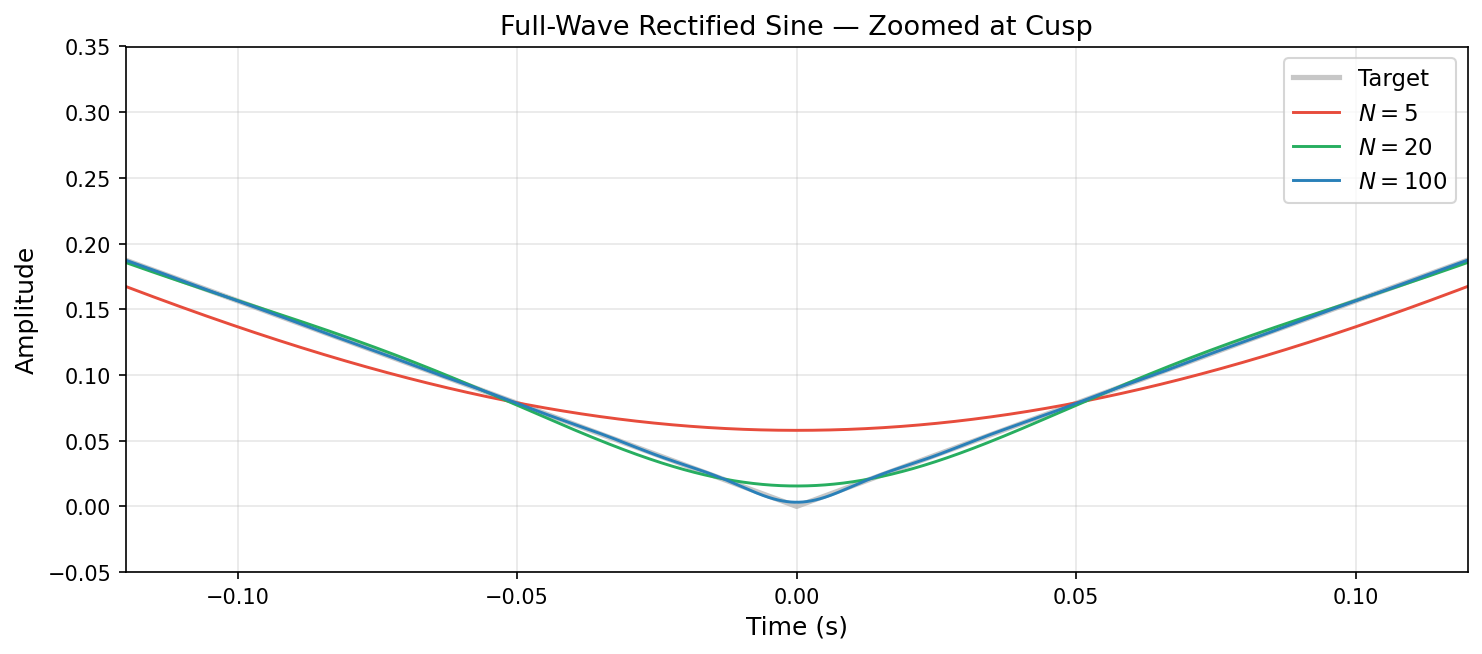
\includegraphics[width=\textwidth,height=0.85\textheight,keepaspectratio]{rect_zoom.png}
\end{frame}

\begin{frame}{Discussion}
\textbf{Fourier Series Formulas Used}
\begin{itemize}
  \item \textbf{Square wave:} $f(t)=\dfrac{4}{\pi}\displaystyle\sum_{n=1,3,5,\ldots}^{N}\dfrac{1}{n}\sin(n\omega_0 t)$ \quad (odd harmonics, coefficients $\propto 1/n$)
  \item \textbf{Triangular wave:} $f(t)=\dfrac{8}{\pi^2}\displaystyle\sum_{n=1,3,5,\ldots}^{N}\dfrac{(-1)^{(n-1)/2}}{n^2}\sin(n\omega_0 t)$ \quad (coefficients $\propto 1/n^2$)
  \item \textbf{Rectified sine:} $f(t)=\dfrac{2}{\pi}-\dfrac{4}{\pi}\displaystyle\sum_{n=1}^{N}\dfrac{1}{4n^2-1}\cos(n\omega_0 t)$ \quad (DC + cosine terms)
\end{itemize}

\bigskip
\textbf{Q1. Does the Gibbs phenomenon occur?}
\begin{itemize}
  \item \textbf{Square wave -- Yes.} Every jump discontinuity (at $t=0,\,T/2,\,T,\ldots$) produces $\approx9\%$ overshoot. Ringing is clearly visible in the zoom slide.
  \item \textbf{Triangular wave -- No.} Continuous everywhere; only the \emph{derivative} is discontinuous at peaks/valleys. No ringing observed.
  \item \textbf{Rectified sine -- No.} Continuous everywhere; only the slope is discontinuous at the cusps. No ringing observed.
\end{itemize}

\bigskip
\textbf{Q2. Overshoot ratio (overshoot / step height):}
$\quad\dfrac{1.18-1.00}{2.00}\approx\mathbf{9\%}$ for the square wave; $\approx0$ for the other two.

\bigskip
\textbf{Q3. Does the overshoot disappear as $N\to\infty$?}\quad\textbf{No.}
The spike narrows but its \emph{height remains} $\approx9\%$ for all finite $N$ -- this is the Gibbs phenomenon.
\end{frame}

\begin{frame}{Discussion: Sinc Function, Square Wave, and Gibbs Phenomenon}
\textbf{Q4. Mathematical connection between sinc, square wave, and Gibbs phenomenon}

\begin{itemize}
  \item \textbf{Frequency truncation $\equiv$ rect window.}
  Keeping only $N$ harmonics multiplies the Fourier spectrum by a rectangular (rect) function centered at zero.

  \item \textbf{Convolution theorem.}
  Multiplication in frequency $\Longleftrightarrow$ convolution in time:
  \[
    \mathcal{F}^{-1}\!\bigl\{\mathrm{rect}\tfrac{f}{2Nf_0}\bigr\} \propto \mathrm{sinc}(2Nf_0\,t)
    \quad\Longrightarrow\quad S_N(t) = f(t) * \mathrm{sinc}(2Nf_0\,t)
  \]

  \item \textbf{Sinc side lobes cause ringing.}
  The sinc kernel has infinitely many decaying side lobes. Convolving a step discontinuity with this kernel smears the jump and produces oscillatory over/undershoot on both sides.

  \item \textbf{Fixed 9\% overshoot.}
  The first positive side lobe always contributes the same fractional area, giving a permanent overshoot:
  \[
    \lim_{N\to\infty}\max S_N(t) = 1 + \frac{1}{\pi}\int_0^{\pi}\frac{\sin u}{u}\,du - 1 \approx 0.0895
  \]

  \item \textbf{Conclusion.}
  As $N\to\infty$ the sinc narrows toward $\delta(t)$ (perfect reconstruction everywhere except at the jump), but for any \emph{finite} $N$ the side lobes persist --- which is why the Gibbs overshoot \textbf{never disappears}.
\end{itemize}
\end{frame}

\end{document}
